\section{Painel Integrado de Transitórios Eletromecânicos}\label{sec:painel_transitorios}

A avaliação unificada das trajetórias dinâmicas registradas nos três cenários de simulação proporciona uma perspectiva abrangente acerca dos tempos de resposta eletromecânicos e da estabilidade de integração numérica do modelo Simscape SPS. A justaposição em painel contínuo evidencia a transição suave entre a partida a vazio, a acomodação sob choque mecânico de carga nominal e a reversão de fluxo energético no regime regenerativo hipersíncrono.

% =========================================================================
% [DIRETRIZ DE REDAÇÃO]
% - Objetivo: Apresentar o painel consolidado de transitórios multimodais, integrando
%   as respostas temporais de partida direta a vazio, degrau de carga e frenagem regenerativa.
% - Formulação: Discutir as transições entre quadrantes de operação mecânica e elétrica
%   (motor subsíncrono vs. gerador hipersíncrono) em uma escala temporal unificada.
% - Figuras/Tabelas: Inserir a figura em largura de página inteira: consolidated_transient_overview.png.
% - Confronto: Avaliar o tempo de resposta mecânico em função da inércia pesada acoplada (J = 0,701 kg*m^2).
% =========================================================================

A \Cref{fig:painel_consolidado} apresenta o painel integrado de transitórios dinâmicos do Simscape Specialized Power Systems, reunindo em escala temporal síncrona a velocidade, o conjugado, a corrente eficaz de estator e as potências ativa e reativa para todos os regimes estudados.

\begin{figure}[H]
\centering
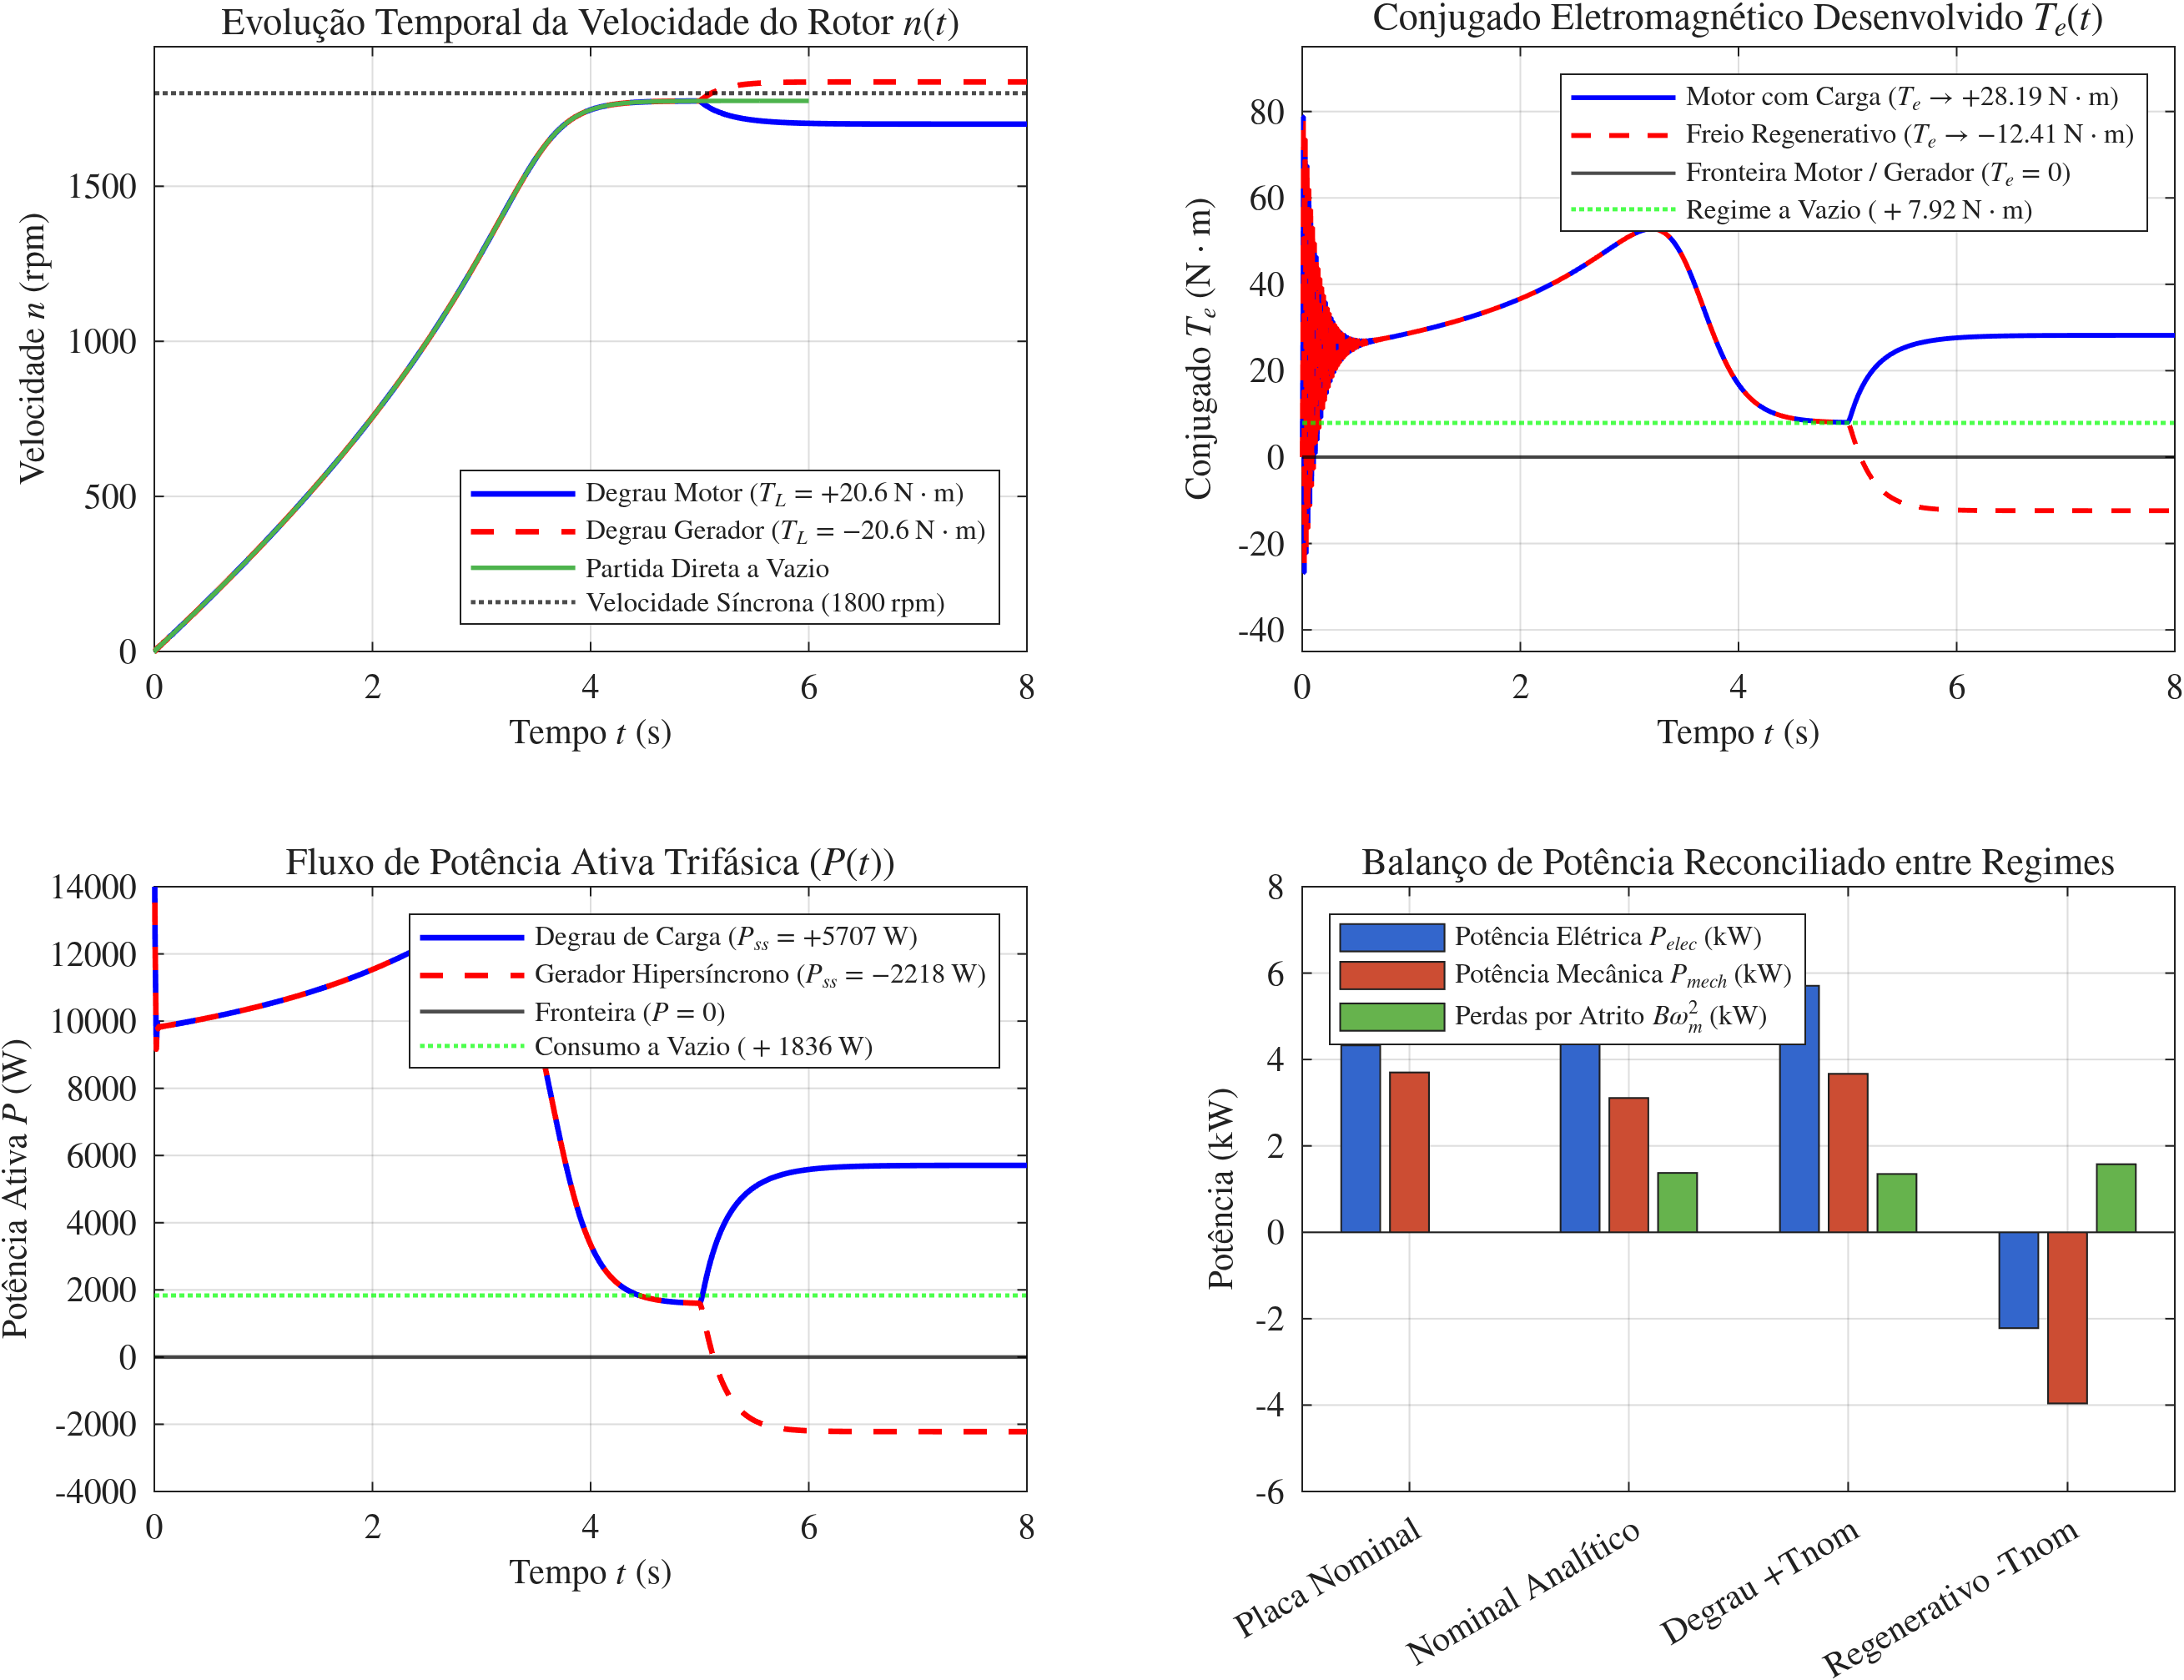
\includegraphics[width=\textwidth]{consolidated_transient_overview.png}
\caption{Painel sinóptico de transitórios eletromecânicos da máquina de indução simulada no Simscape SPS.}
\label{fig:painel_consolidado}
\end{figure}

O painel atesta a robustez do solver L-estável na transição entre os quadrantes operacionais e confirma a estabilidade das variáveis após a extinção das oscilações subtransitórias elétricas e mecânicas.
